\documentclass[
   %handout
 ]{beamer}
 
\usetheme{simple}
\usepackage{lmodern}
\usepackage[scale=2]{ccicons}

%Codifica dei font di input e di output
\usepackage[T1]{fontenc}
\usepackage[utf8]{inputenc}

% Converte file eps in pdf
\usepackage{epstopdf}

% Consente di impostare le virgolette del discorso diretto
\usepackage{dirtytalk}

% Consente di impostare i commenti multiline
\usepackage{verbatim}

% Consente di disegnare grafi
\usepackage{tikz}

% Libreria per disegnare cerchi e frecce di tikz
\usetikzlibrary{arrows}

% Definizione della cartella contenente le immagini da usare
\graphicspath{{img/}}

% Disabilitare la trasparenza sulla pause
\setbeamercovered{invisible}


% TODO
% Migliorare la spiegazione delle slide


% Watermark background (simple theme)

%\setwatermark{\includegraphics[height=8cm]{img/Heckert_GNU_white.png}}


\title{Implementazione di una \\ 
       Rete Convoluzionale in CUDA 
       \texorpdfstring{\bigskip}{Lg}
      }
      
\author{\hspace*{0.01em} {\Large Michele Valsesia} 
                         \texorpdfstring{\\ \bigskip}{Lg}
        \hspace*{-0.11em}{\Large Nicholas Aspes}
       }
       
\date{\Large Anno accademico 2018/2019}
%\institute{\url{http://github.com/famuvie}}

\begin{document}

\maketitle



% //////////////////////////////// Introduzione ////////////////////////////////////////
\begin{frame}{Introduzione}
    \framesubtitle{Obiettivi}  
    
    \begin{itemize} [<+->]
        \setlength\itemsep{2em}
        \item \large Descrivere brevemente l'architettura ed il funzionamento di una\emph{Rete Neurale}
        \item \large Motivare le differenti scelte implementative adottate durante lo svolgimento del progetto
        \item \large Valutare l'accuratezza e lo speed-up della rete rispetto ad una sua implementazione sequenziale       
    \end{itemize}  
\end{frame}


% //////////////////////////////// Parte Teorica Reti Neurali //////////////////////////

\begin{frame}[c]
  \centering
  \bigskip \bigskip    
  \Huge Reti Neurali
\end{frame}

\begin{frame}{Reti Neurali}
    \framesubtitle{Motivazioni Biologiche}
    \begin{itemize} [<+->]
        \setlength\itemsep{2em}
        \item \large Una \emph{Rete Neurale} ha come scopo quello di modellare una rete neurale biologica
       \item \large Una rete neurale biologica si compone di unità cellulari di base: i \emph{neuroni}
       \item \large I neuroni sono collegati tra loro per mezzo di specifiche giunture chiamate \emph{sinapsi}
    \end{itemize}
\end{frame} 

\begin{frame}{Reti Neurali}
    \framesubtitle{Neurone}
    
    \begin{center}
      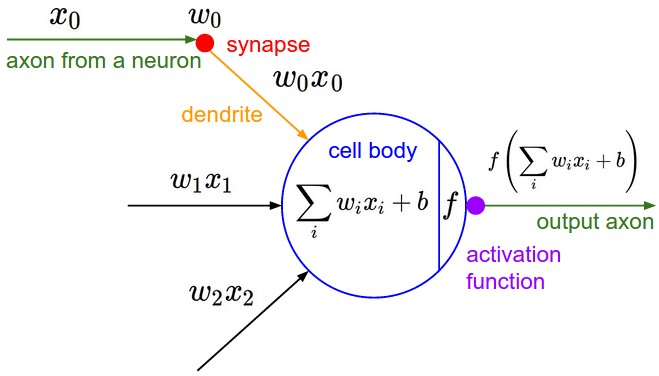
\includegraphics[scale = 0.4]{neuron_model.jpeg}
    \end{center}
  
    \bigskip 
  
  \begin{itemize}
    \setlength\itemsep{1em}
    \item[] \large \emph{Modello matematico di un neurone}
  \end{itemize}       
\end{frame} 


\begin{frame}{Reti Neurali}
    \framesubtitle{Funzionamento Neurone}
    \begin{itemize} [<+->]
        \setlength\itemsep{2em}
        \item \large Attraverso un meccanismo di eccitazione ed inibizione i pesi sinaptici controllano quanto un neurone sia influenzato dagli altri
       \item \large I segnali pesati dalle differenti sinapsi vengono trasportati dai dendriti all'interno del neurone e sommati tra loro
       \item \large Se la somma supera una certa soglia, il neurone \emph{spara} un segnale lungo l'assone 
       \item \large La \emph{frequenza di sparo} del neurone viene modellata con una funzione di attivazione $f$       
    \end{itemize}
\end{frame}

% Funzioni di attivazione

\begin{frame}{Reti Neurali}
    \framesubtitle{Rete Neurale}
    
    \begin{block}{Definizione} 
        \large Una \emph{Rete Neurale} è composta da un insieme di neuroni connessi in un grafo aciclico. I neuroni sono organizzati come una serie di livelli (layer) distinti.
    \end{block}\pause
    \begin{itemize} [<+->]
        \setlength\itemsep{2em}
        \item \large Attraverso un meccanismo di eccitazione ed inibizione i pesi sinaptici controllano quanto un neurone sia influenzato dagli altri
       \item \large I segnali pesati dalle differenti sinapsi vengono trasportati dai dendriti all'interno del neurone e sommati tra loro
       \item \large Se la somma supera una certa soglia, il neurone \emph{spara} un segnale lungo l'assone 
       \item \large La \emph{frequenza di sparo} del neurone viene modellata con una funzione di attivazione $f$       
    \end{itemize}
\end{frame}




\begin{frame}{Reti Neurali}
    \framesubtitle{Rete Neurale Convoluzionale}  
    Una \emph{Rete Neurale Convoluzionale} si differenzia da una più classica in quanto assume che l'input della rete sia un'immagine
\end{frame}   

\begin{frame}[c]
  \centering
  \bigskip \bigskip    
  \Huge Implementazione della Rete
\end{frame}

\begin{frame}[c]
  \centering
  \bigskip \bigskip    
  \Huge Analisi dei Risultati
\end{frame}


\end{document}
